\section{Ontology-Enhanced RAG Framework}
\label{sec:framework}

This section presents the ontology construction process and its integration into the RAG pipeline. Section~\ref{ssec:formal} gives formal definitions. Section~\ref{ssec:hierarchy} describes the ingredient hierarchy and dish taxonomy. Section~\ref{ssec:relations} details relation derivation. Section~\ref{ssec:integration} explains the three ontology injection points.

% ──────────────────────────────────────────────────────────────
\subsection{Formal Definition}
\label{ssec:formal}

We define the food ontology as a tuple $\mathcal{O} = (\mathcal{C}, \mathcal{R}, \mathcal{I}, \mathcal{A})$, where $\mathcal{C}$ is a set of classes organized in a rooted tree (T-box), $\mathcal{R}$ is a set of named relation types, $\mathcal{I}$ is a set of instances (ingredients and dishes), and $\mathcal{A}$ is a set of assertions linking instances to classes and to each other (A-box). The class hierarchy supports the \emph{subClassOf} relation: if $c_1 \sqsubseteq c_2$, then every ingredient in $c_1$ is also in $c_2$. Table~\ref{tab:relations} lists the seven named relations with their derivation sources and corpus-level counts.

\begin{table}[t]
\centering
\caption{Named relations in the food ontology.}
\label{tab:relations}
\small
\begin{tabular}{llll}
\toprule
\textbf{Relation} & \textbf{Signature} & \textbf{Derivation} & \textbf{Count} \\
\midrule
hasIngredient      & dish $\times$ ing            & direct from KB     & 10{,}741 \\
mainIngredient     & dish $\times$ ing            & importance $\geq$ 3 & 10{,}741 \\
subClassOf         & class $\times$ class         & manual curation    & 49 \\
substitutes        & ing $\times$ ing $\times$ ctx & dish-name diff    & 5{,}407 \\
flavorComplements  & ing $\times$ ing             & NPMI $>$ 0.3      & 15{,}119 \\
conflictsWith      & ing $\times$ ing             & curated rules      & 139 \\
cookedBy           & dish $\times$ method         & category pattern   & 10{,}741 \\
\bottomrule
\end{tabular}
\end{table}

% ──────────────────────────────────────────────────────────────
\subsection{Ingredient Hierarchy and Dish Taxonomy}
\label{ssec:hierarchy}

\textbf{Ingredient hierarchy.}
The ingredient hierarchy is a four-level rooted tree with 49 classes (39 leaf classes) covering 8{,}112 Vietnamese ingredients. Level~0 is the root \texttt{Ingredient}; Level~1 contains nine top categories (\texttt{Protein}, \texttt{Produce}, \texttt{Seasoning}, \texttt{Staple}, \texttt{Dairy}, \texttt{Beverage}, \texttt{Sweet}, \texttt{Processed}, \texttt{Other}); Level~2 and Level~3 provide finer distinctions (e.g., \texttt{Protein} $\to$ \texttt{AnimalProtein} $\to$ \texttt{Seafood}). Construction follows a two-stage process: (1)~manual design of the class tree based on Vietnamese culinary conventions, and (2)~automated classification of each ingredient into a leaf class using an LLM classifier (Qwen-2.5 7B, temperature~0, batch size~25), with manual validation of the 100 most frequent ingredients and spot-checking of 50 random samples. Ingredients that cannot be resolved are assigned to a fallback \texttt{Other} class. Fig.~\ref{fig:hierarchy} illustrates the top three levels.

% --- FIGURE: Hierarchy tree ---
\begin{figure}[t]
\centering
% 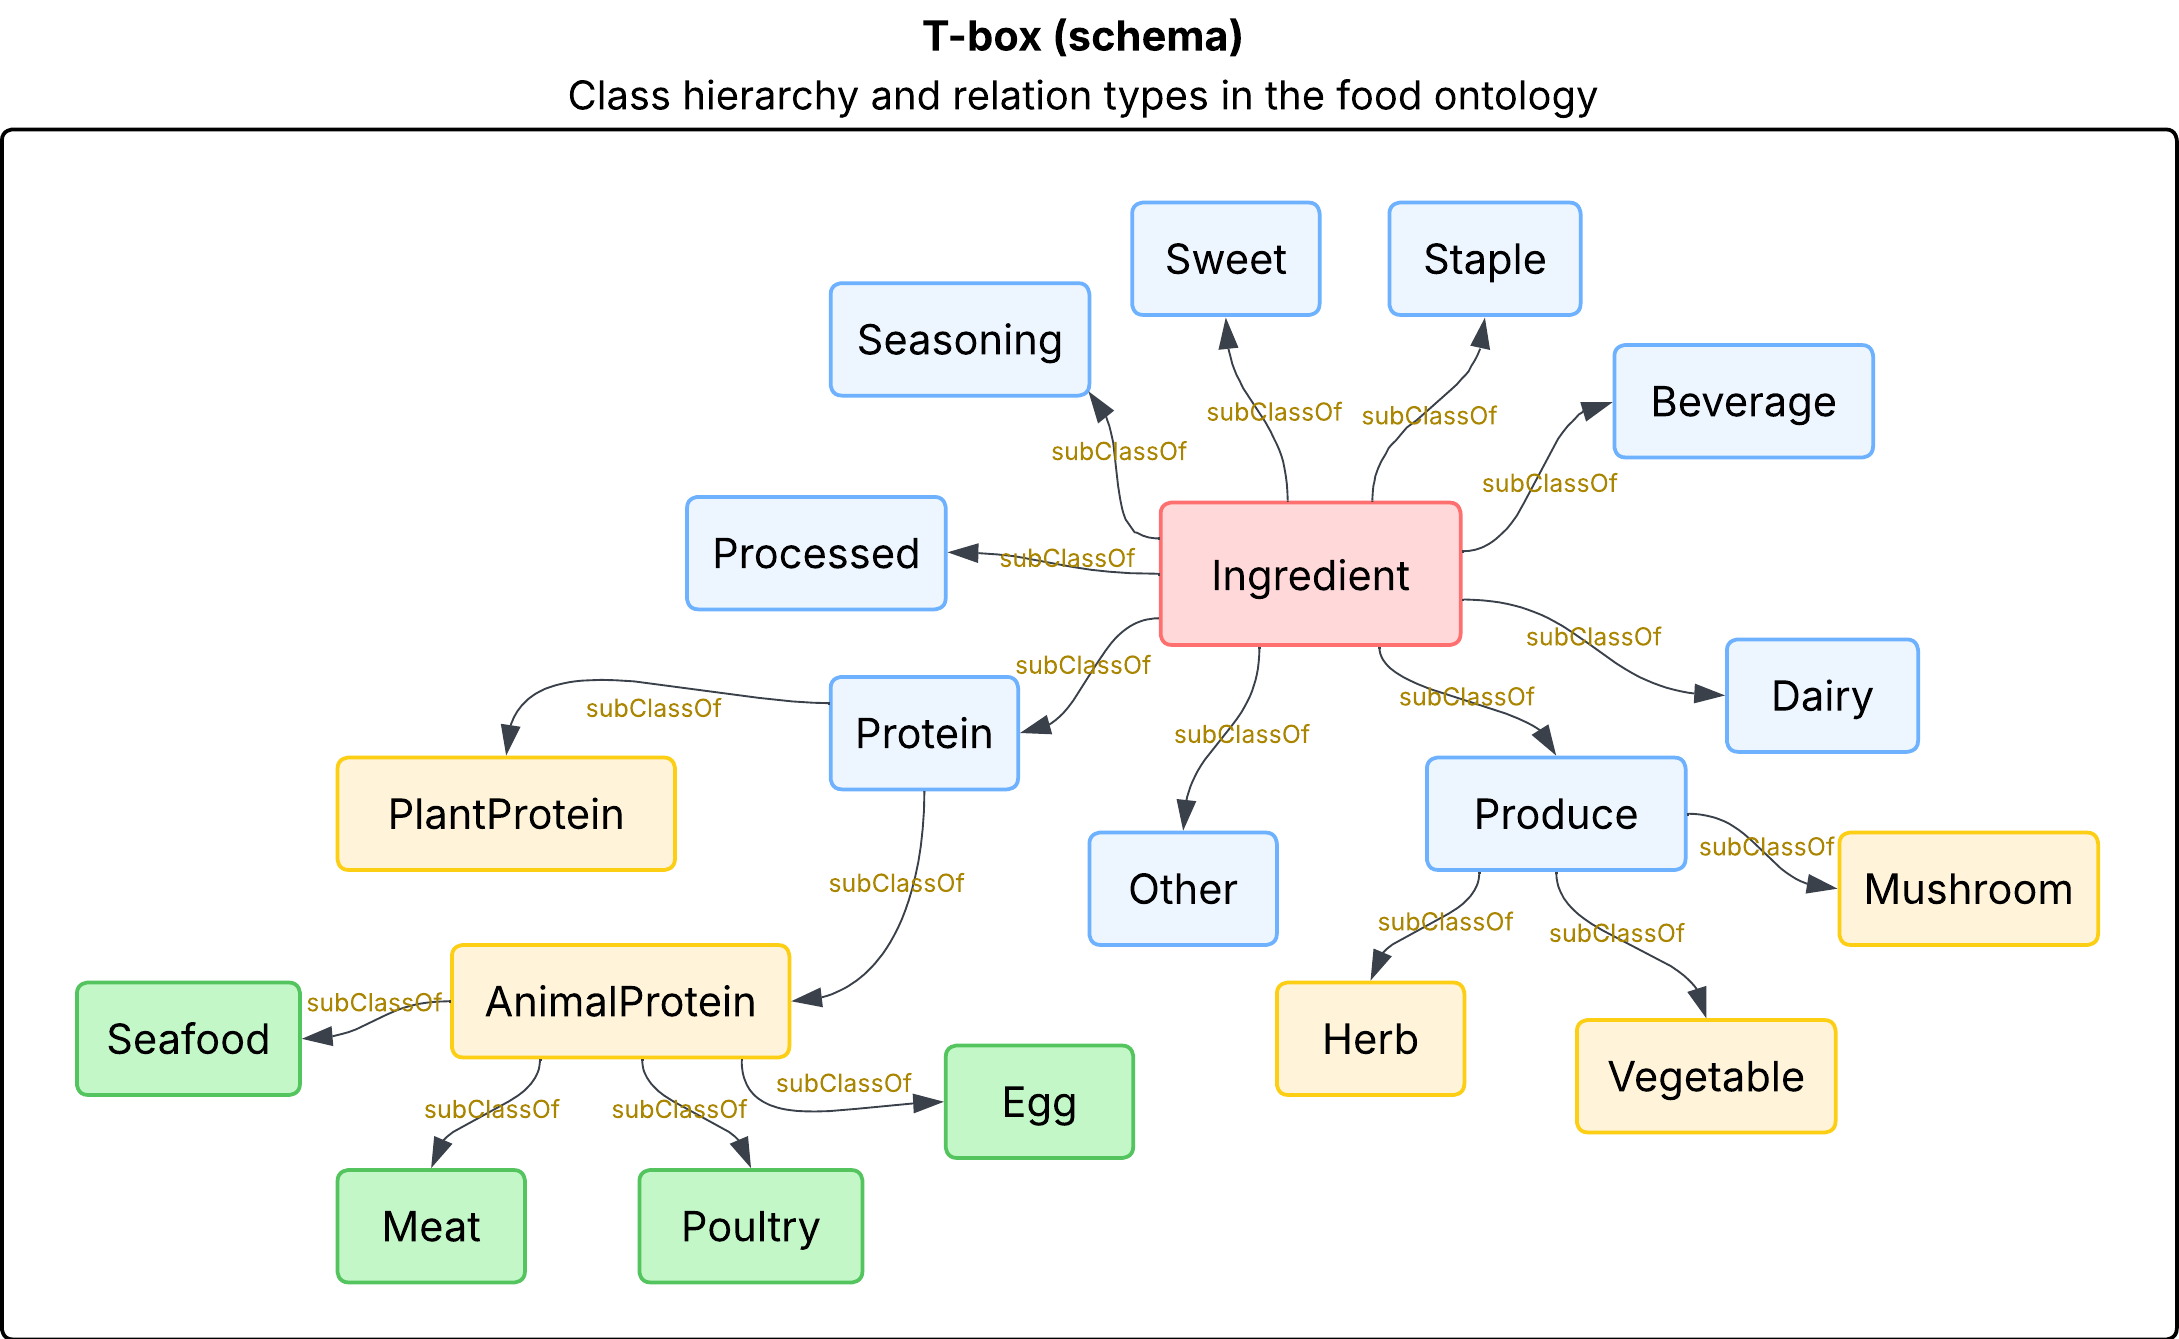
\includegraphics[width=\columnwidth]{figures/hierarchy_tree.pdf}
\fbox{\parbox{0.92\columnwidth}{\centering\small
\texttt{Ingredient} (8{,}112)\\[2pt]
\texttt{Protein} (1{,}273) \quad \texttt{Produce} (1{,}834) \quad \texttt{Seasoning} (2{,}508) \quad \texttt{Staple} (571) \quad \ldots\\[2pt]
\texttt{AnimalProtein} \quad \texttt{PlantProtein}(69) \quad \texttt{Herb}(402) \quad \texttt{Vegetable}(591) \quad \ldots\\[2pt]
\texttt{Seafood}(519) \quad \texttt{Meat}(333) \quad \texttt{Poultry}(85) \quad \texttt{Egg}(46) \quad \ldots
}}
\caption{Top three levels of the ingredient hierarchy (counts in parentheses).}
\label{fig:hierarchy}
\end{figure}

\textbf{Dish taxonomy.}
Dishes are classified along two orthogonal axes. The \emph{byType} axis groups dishes into 15 culinary categories (e.g., \texttt{mon\_canh}, \texttt{mon\_kho}, \texttt{mon\_xao}, \texttt{mon\_nuong}). The \emph{byMethod} axis maps each category to one of 15 cooking-method labels (e.g., \texttt{Boil}, \texttt{Stew}, \texttt{StirFry}, \texttt{Grill}), derived from the dish category field via pattern matching. All 10{,}741 dishes receive a cooking-method assignment.

% ──────────────────────────────────────────────────────────────
\subsection{Relation Derivation}
\label{ssec:relations}

Each relation is derived from existing data artifacts rather than manual annotation.

\textbf{substitutes($A$, $B$, context).}
We identify dish pairs whose names differ by exactly one content token (e.g., ``Ph\h{o} b\`{o}'' vs.\ ``Ph\h{o} g\`{a}''). If the differing tokens correspond to main ingredients, those ingredients are recorded as substitutes in the context of the shared name template. This yields 5{,}407 substitution pairs grounded in actual Vietnamese dish variation.

\textbf{flavorComplements($A$, $B$).}
We compute Normalized Pointwise Mutual Information (NPMI) over ingredient co-occurrence across all 10{,}741 dishes:
%
\begin{equation}
\label{eq:npmi}
\text{NPMI}(A, B) = \frac{\log \frac{P(A, B)}{P(A)\,P(B)}}{-\log P(A, B)}
\end{equation}
%
All pairs with $\text{NPMI} > 0.3$ are retained, yielding 15{,}119 complement pairs. No additional class filter is applied at derivation time; class-based filtering is performed downstream during substitution reasoning (Section~\ref{ssec:integration}).

\textbf{conflictsWith($A$, $B$).}
139 nutritional and medical conflict rules are imported from an existing curated conflict database and normalized to ontology ingredient identifiers.

\textbf{cookedBy(dish, method).}
The cooking method is mapped from the dish category field using a 15-entry lookup table (e.g., ``m\'{o}n x\`{a}o'' $\to$ \texttt{StirFry}), covering all 10{,}741 dishes.

% ──────────────────────────────────────────────────────────────
\subsection{Ontology Integration with RAG}
\label{ssec:integration}

The ontology is injected into the dense-retrieval RAG pipeline at three points, each targeting one of the failure modes identified in Section~\ref{sec:introduction}. Fig.~\ref{fig:pipeline} illustrates the overall architecture.

% --- FIGURE: Pipeline ---
\begin{figure}[t]
\centering
% 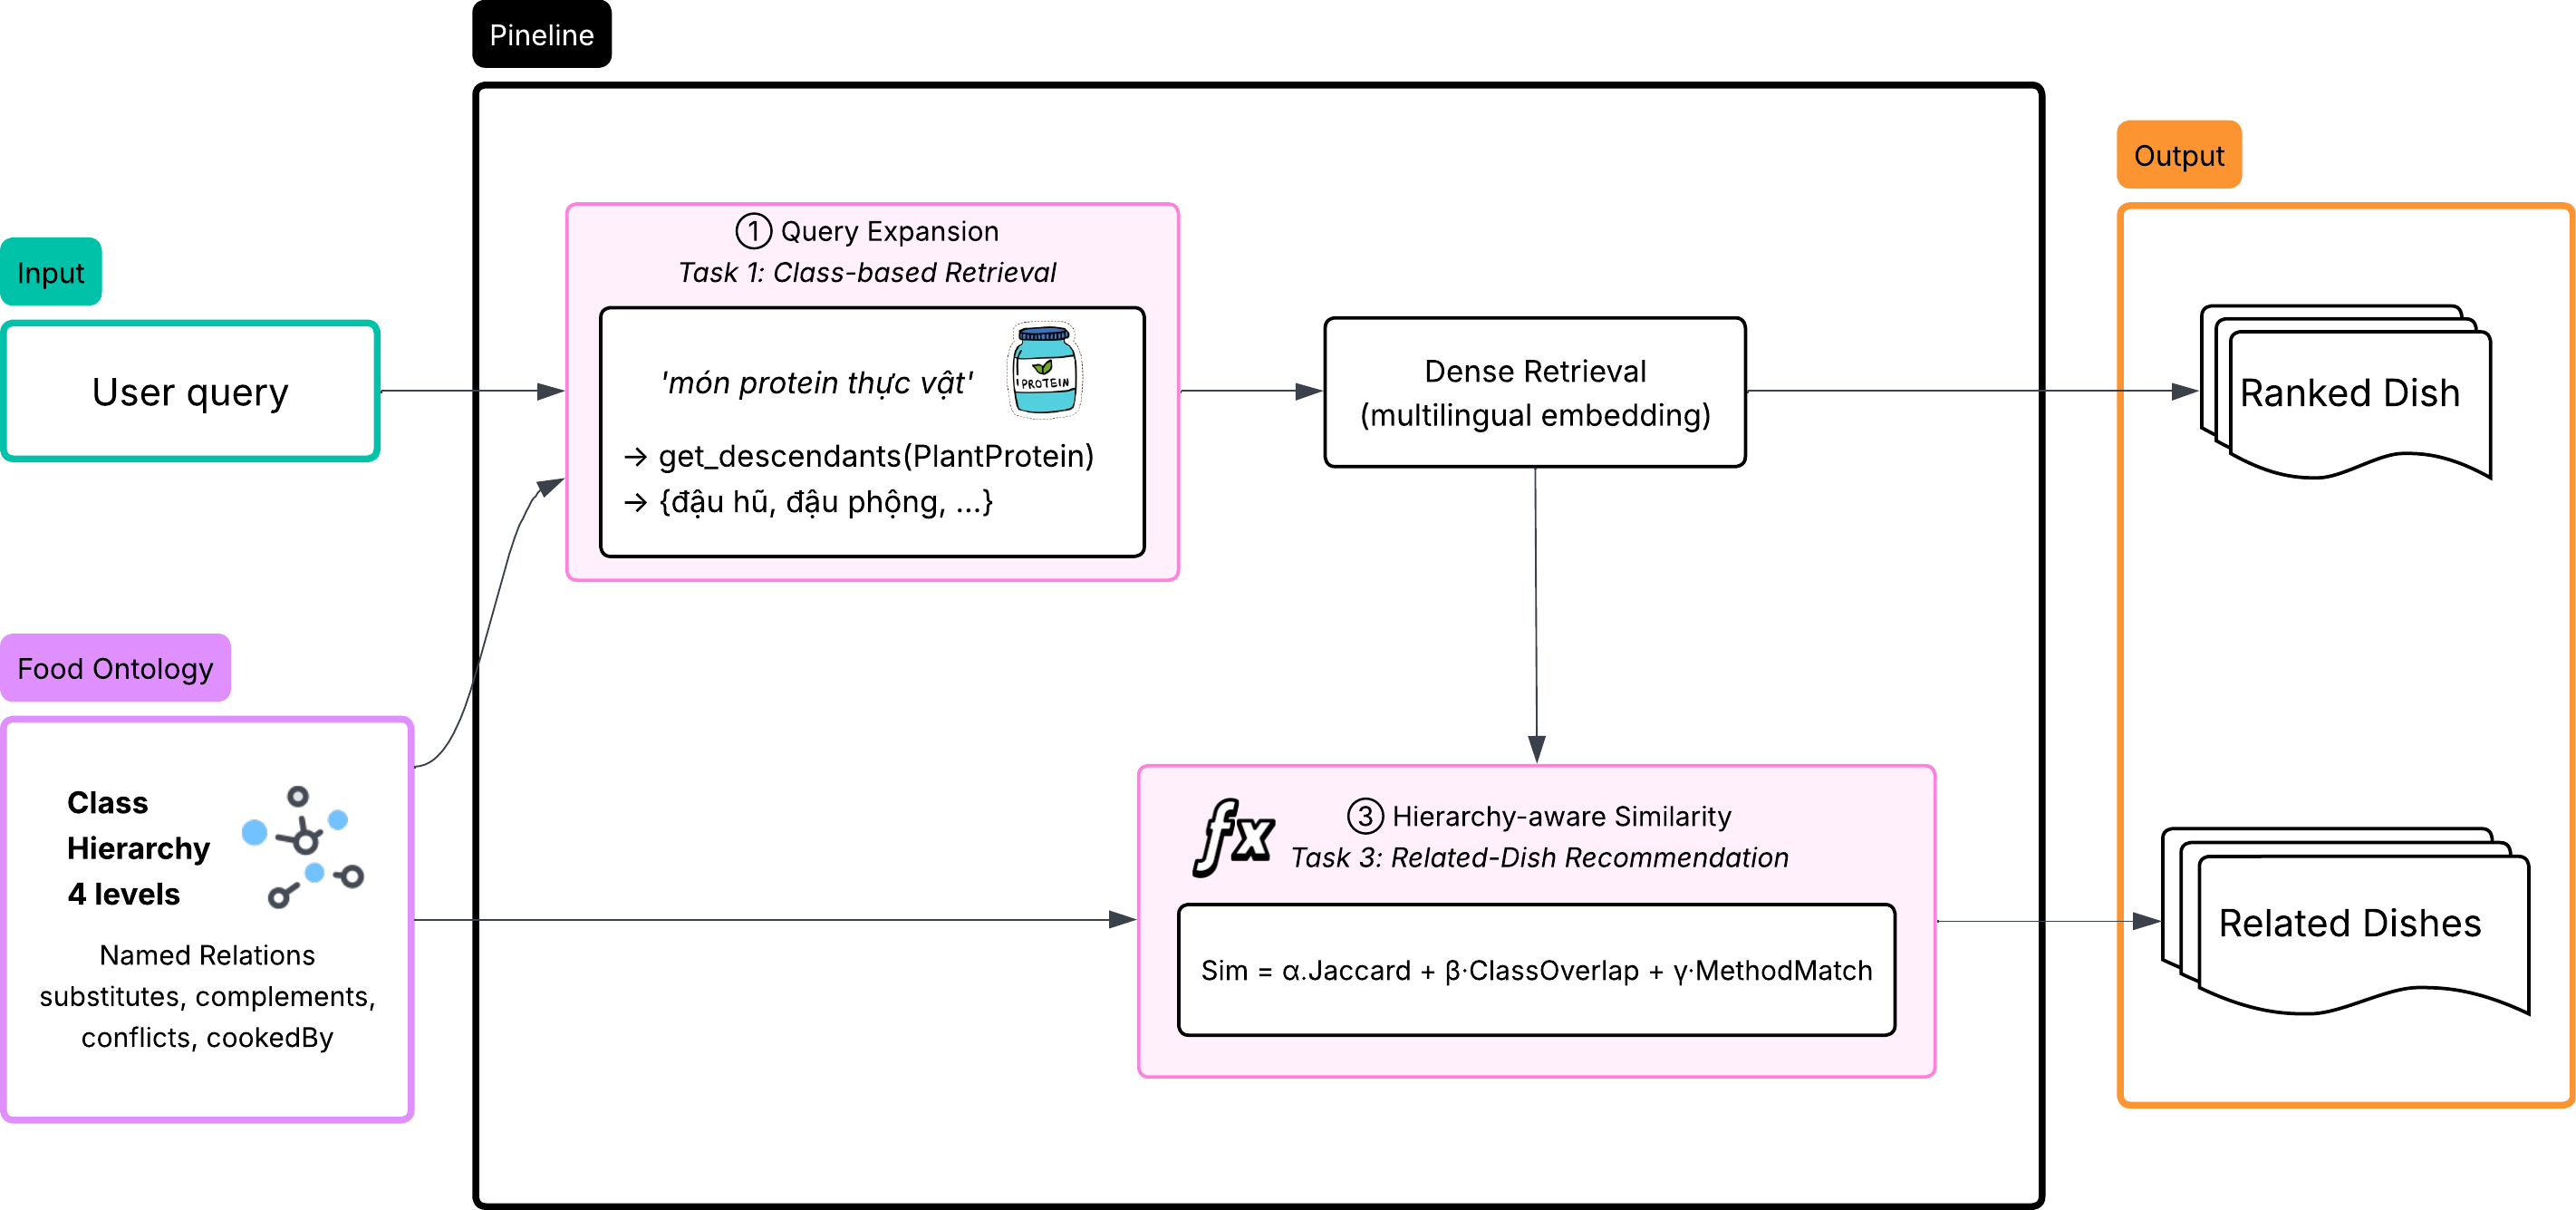
\includegraphics[width=\columnwidth]{figures/pipeline.pdf}
\fbox{\parbox{0.92\columnwidth}{\centering\small
\textbf{Query} $\xrightarrow{\text{(1) expand}}$ Expanded Query $\xrightarrow{\text{dense retrieval}}$ Candidates\\[4pt]
\textbf{Substitution request} $\xrightarrow{\text{(2) lookup + filter}}$ Ranked substitutes\\[4pt]
\textbf{Dish} $\xrightarrow{\text{(3) hierarchy-aware sim}}$ Related dishes
}}
\caption{Ontology injection points in the RAG pipeline.}
\label{fig:pipeline}
\end{figure}

\textbf{(1) Query expansion (Task~1).}
For class-level queries such as \textit{``m\'{o}n protein th\d{u}c v\d{a}t''}, the system maps the class term to an ontology node and retrieves all descendant ingredient names via \texttt{get\_descendants}. The expanded ingredient list is appended to the original query before dense encoding. Negation queries (e.g., ``m\'{o}n kh\^{o}ng h\h{a}i s\h{a}n'') expand the positive class and exclude matching dishes at retrieval time.

\textbf{(2) Constrained substitution reasoning (Task~2).}
Given a dish, a target ingredient, and a dietary constraint (e.g., vegetarian), the system: (a)~looks up \emph{substitutes} relations filtered by dish context, (b)~expands candidates to same-class and sibling-class members, (c)~filters candidates through the class hierarchy (e.g., vegetarian $\to$ exclude \texttt{AnimalProtein} descendants), and (d)~ranks survivors by NPMI compatibility with the remaining dish ingredients:
%
\begin{equation}
\label{eq:sub_score}
\text{Score}(c) = \text{NPMI}_{\text{avg}}(c, \text{others}) + \lambda_1 \cdot \mathbb{1}[\text{ont\_sub}] + \lambda_2 \cdot \mathbb{1}[\text{same\_leaf}]
\end{equation}
%
where $\lambda_1 = 0.3$ and $\lambda_2 = 0.2$ are bonus weights for ontology-attested substitutes and same-leaf-class candidates, respectively.

\textbf{(3) Hierarchy-aware dish similarity (Task~3).}
Dish similarity combines four components:
%
\begin{equation}
\label{eq:sim}
\text{Sim}(A, B) = \alpha \cdot J + \beta \cdot C + \gamma \cdot M + \delta \cdot S
\end{equation}
%
where $J = \text{Jaccard}(A, B)$ is standard set overlap on ingredient IDs; $C = \text{ClassOverlap}(A, B)$ uses greedy bipartite matching over ingredient classes (same-leaf $\to$ 1.0, same-parent $\to$ 0.5, normalized by $\max(|A|, |B|)$); $M = \text{MethodMatch}(A, B)$ returns 1.0 if both dishes share the same cooking method; and $S = \text{SemanticSim}(A, B)$ captures pre-computed ingredient-level semantic similarity from embedding-based matrices. Weights are tuned on a 50-pair development set to maximize Pearson correlation with human-judged relatedness, yielding $\alpha = 0.50$, $\beta = 0.25$, $\gamma = 0.15$, $\delta = 0.10$.
